\ifx\boi\undefined\ifx\problemname\undefined
\providecommand\sampleinputname{}
\providecommand\sampleoutputname{}
\documentclass[english]{templates/boi}
\problemlanguage{.en}
\fi
\newcommand{\boi}{Baltic Olympiad in Informatics}
\newcommand{\practicesession}{Practice Session}
\newcommand{\contestdates}{April 27 - May 1, 2018}
\newcommand{\dayone}{Day 1}
\newcommand{\daytwo}{Day 2}
\newcommand{\licensingtext}{This problem is licensed under CC BY-SA 4.0.}
\newcommand{\problem}{Problem}
\newcommand{\inputsection}{Input}
\newcommand{\outputsection}{Output}
\newcommand{\interactivity}{Interactivity}
\newcommand{\grading}{Grading}
\newcommand{\scoring}{Scoring}
\newcommand{\constraints}{Constraints}
\renewcommand{\sampleinputname}{Sample Input}
\renewcommand{\sampleoutputname}{Sample Output}
\newcommand{\sampleexplanation}[1]{Explanation of Sample #1}
\newcommand{\sampleexplanations}{Explanation of Samples}
\newcommand{\timelimit}{Time Limit}
\newcommand{\memorylimit}{Memory Limit}
\newcommand{\seconds}{s}
\newcommand{\megabytes}{MB}
\newcommand{\group}{Group}
\newcommand{\points}{Points}
\newcommand{\limitsname}{Limits}
\newcommand{\additionalconstraints}{Additional Constraints}
\newcommand{\testgroups}{
Your solution will be tested on a set of test groups, each worth a number of points.
Each test group contains a set of test cases.
To get the points for a test group you need to solve all test cases in the test group.
Your final score will be the maximum score of a single submission.
}
\fi
\def\version{jury-1}
\problemname{Teed}
{\em Graaf} on matemaatiline struktuur, mis koosneb hulgast {\em tippudest} ja hulgast {\em servadest}, millest igaüks ühendab kaht serva. 
Allpool on toodud $4$ tipu ja $3$ servaga graafi kirjeldus.
%Näiteks teedekaart võib olla graaf, kui tippudeks on linnad ja servadeks teed, mis linnu otse ühendavad. 

{\em Tee} on defineeritud kui $2$ või enam tipuga järjend, kus järjestikuste tippude vahel on servad. Siin ülesandes huvitavad meid ainult lihtsad teed, see tähendab sellised teed,
kus ükski tipp ei esine rohkem kui ühe korra.
Pane tähele, et järjend on sorteeritud: näiteks järjendid ``\texttt{1-2-3}'', ``\texttt{1-3-2}'' ja ``\texttt{3-2-1}'' on erinevad teed.

Siin ülesandes on antud graaf, mille iga tipp on värvitud ühega $K$ värvist. Tarvis on leida erinevate {\em teede} arv, kus ei leiduks kaht sama värviga värvitud tippu.

\section*{\inputsection}
Sisendi esimesel real on kolm täisarvu: $N$ (tippude arv), $M$ (servade arv) ja $K$ (erinevate värvide arv).

%($1 \le N, M \le 3 \cdot 10^5, 1 \le K \le 5$).

Teisel real on $N$ täisarvu lõigust $1$ kuni $K$, mis tähistavad iga tipu värvi (alustades tipust number $1$ ja lõpetades tipuga number $N$). 

Igaüks järgmistest $M$ reast kirjeldab üht serva ja sellel on kaks täisarvu $a, b$ ($1 \le a, b \le N, a \neq b$) -- vastava servaga ühendatud tippude numbrid. 
Iga tipupaari vahel on ülimalt üks serv.

\section*{\outputsection}
Väljastada üks täisarv: erinevate teede arv, kus sama tee raames on kõik tipud eri värvi. Vastus on alati väiksem kui $10^{18}$.

\section*{\constraints}
\testgroups

\noindent
\begin{tabular}{| l | l | l |}
\hline
\group & \points & \limitsname \\ \hline
1      & 23      & $1 \le N, M \le 100, 1 \le K \le 4$ \\ \hline
2      & 20      & $1 \le N, M \le 300\,000, 1 \le K \le 3$ \\ \hline
3      & 27      & $1 \le N, M \le 300\,000, 1 \le K \le 4$ \\ \hline
4      & 30      & $1 \le N, M \le 100\,000, 1 \le K \le 5$ \\ \hline
\end{tabular}

\section*{\sampleexplanation{1}}

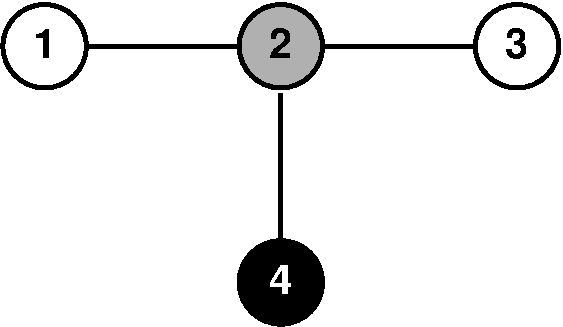
\includegraphics[width=5cm]{pathsfig.pdf}

Esimeses näites kirjeldatud graaf on toodud joonisel, kus iga tipp on kas valge (värv 1), hall (värv 2) või must (värv 3). 
Graafis leidub 10 teed, mille kõik tipud on erinevat värvi: ``\texttt{1-2}'', ``\texttt{2-1}'', ``\texttt{2-3}'', ``\texttt{3-2}'', ``\texttt{2-4}'', ``\texttt{4-2}'', ``\texttt{1-2-4}'', ``\texttt{4-2-1}'', ``\texttt{3-2-4}'' ja ``\texttt{4-2-3}''.

Pane tähele, et ``\texttt{1}'' ei ole tee, sest seal on ainult üks tipp, ning ``\texttt{1-2-3}'' ei ole lubatud tee, sest selles on kaks tippu värviga $1$.
